\documentclass[final,a4paper,11pt,notitlepage,halfparskip]{scrreprt}

\usepackage[german,ngerman]{babel}
\usepackage[utf8]{inputenc}
\usepackage[T1]{fontenc}
\usepackage[babel,german=quotes]{csquotes}
%\usepackage{fancybox}
%\usepackage{color}
\usepackage{xcolor}
\usepackage{hyperref}
%\usepackage{floatflt}
\usepackage{graphicx}
%\usepackage{amsmath}
%\usepackage{amssymb}
%\usepackage{amsfonts}
%\usepackage{listings}

\setkomafont{caption}{\footnotesize\linespread{1}\selectfont}
\setlength{\abovecaptionskip}{-0.1cm}
\addto\captionsngerman{\renewcommand\figurename{Abb.}}

\title{Beleg\\
Rechnernetze/\\
Kommunikationssysteme}
\author{Jan Losinski}

\begin{document}

\maketitle

\tableofcontents

\chapter{Aufgabe}

\section{Wortlaut}
Schreiben Sie einen Daemon, welcher E-Mails per ESMTP annehmen und weiterleiten 
oder speichern sowie dem jeweiligen Nutzer per POP3 zur Verfügung stellen kann. 
Die Implementierung von ESMTP muss eine Authentisierung des Nutzers vor dem 
Absenden erzwingen. Die weitere Implementierung muss E-Mails annehmen und an die 
passende E-Mail-Domain weiterleiten können, falls es sich bei dem Empfänger 
nicht um einen lokalen Nutzer handelt. Das aussenden und Abrufen von E-Mails 
muss mit einem E-Mail-Programm, wie beispielsweise Evolution oder Thunderbird 
möglich sein.

Randbedingungen:
\begin{itemize}
  \item Implementierung in C, nicht C\# oder C++ oder \dots
  \item weitgehende Modularisierung, beispielsweise in einen POP3-Parser etc.
  \item der Daemon läuft als ein Prozess ohne Threads (oder Forks)
  \item das Mailboxformat darf beliebig sein
  \item das Mailboxformat darf beliebig sein
  \item die Anzahl der Nutzer darf auf 5 beschränkt sein
  \item der Daemon muss ohne weiteres auf den Rechnern im Labor S311 übersetzt 
        werden können und dort laufen
  \item Gruppenarbeiten sind nicht erlaubt
  \item Die Dokumentation des Daemons wie auch der Quellen geht in die Bewertung 
        ein
  \item es dürfen Bibliotheken verwendet werden, beispielsweise SQLITE oder 
        GDBM, soweit diese keine grundlegenden Funktionen von POP3 oder (E)SMTP 
	zur Verfügung stellen.
  \item Die Abgabe des Belegs erfolgt über das SVN. Geprüft wird die letzte 
        Revision. Das SVN ist ab 29.01.2009 0:00 nur noch lesbar. Nachreichungen 
	werden nicht akzeptiert.
\end{itemize}

Programmieren sie nicht einfach darauf los. Beginnen Sie mit einer Konzeption 
der benötigten Programmmodule. Diese Konzeption darf (und sollte auch) in 
Gruppenarbeit erstellt werden.

Der Daemon soll mindestend folgende Kommandozeilenparameter unterstützen
\begin{description}
  \item[-h] Dokumentation der Kommandozeilenparameter und exit
  \item[-V] Informationen zur Version, SVN-Revision und Autor (Name, Vorname, Login)
  \item[-p <Portnummer,Portnummer,Portnummer>] Portnummern mit Komma getrennt
            für (E)SMTP, POP3 und POP3S\\ 
            Voreingestellte Portnummern 25,110,995
  \item[-u <Dateiname>] Datei mit den Nutzernamen als CSV-Datei mit "`TAB"' als 
            Feld-Trenner\\ 
	    Format: \texttt{Login\textbackslash tPasswort\textbackslash
	    tsonstiges\dots\textbackslash n}
\end{description} 

\section{Erfragte Zusätze}
Folgende zusätzliche Fahten zur Aufgabenstellung wurden erfragt:
\begin{itemize}
  \item SMTPS soll nicht implementiert werden.
  \item Die Ein/Ausgabe kann blockierend erfolgen.
  \item Der Mailheader muss nicht geparst werden, auch eine Extraktion von
        Mailaddressen muss nicht erfolgen.
  \item Mailrelay soll nur bei authentifiziertem ESMTP möglich sein.
  \item Die Zustellung lokaler Mails ist ohne authehtifizierung möglich. 
\end{itemize}



\chapter{Umsetzung}
\section{Module}
Bei der Planung wurde festgestellt, das eine Aufteilung der funktionalen
Bestandteile des Programmes auf verschiedene getrennte und nur über definierte
Schnittstellen kommunizierende Module sinvoll ist. So können Fehler lokal
begrenzt und schneller gefunden werden. Auch seiteneffekte einer späteren 
Problembehebung können somit auf das bearbeitete Modul begrenzt werden, solang
die Schnittstelle zu den anderen Modulen gleich bleibt. 

Zudem wird der Code übersichtlicher und für dritte einfacher lesbar, da klar
definiert ist, wo nach einer bestimmten Funktionalität zu suchen ist.

Diese Modulaufteilung ist in C leider nur rudimentär umsetzbar, da es keine
echte Kapselung funktionaler Einheiten oder gar Namensräume gibt. Die Wahl einer
anderen Programmiersprache, wie z.B. C++ hätte dies wesentlich vereinfacht und
zusätzlich noch für besser lesbaren Code gesorgt. Auch die Typsicherheit und
eine damit einhergehende Reduzierung der Fehlerwarscheinlichkeit in der
Implementation wären in vielen anderen Sprachen besser gewesen.

Die aus der Aufgabenstellung abgeleiteten Funktionalitäten, welche jeweils in
einem eigenständigem Modul zusammen gefasst sind zeigt die folgende Tabelle.
Zudem ist in Abb \ref{fig:schema} eine Übersicht über die Module und ihr
Zusammenspiel zu sehen.

Die Implementierungen der Module befinden sich jeweils in einer eigenen C-Datei,
welche den Namen des Moduls trägt. Die Schnittstellen sind in den gleichnamigen
Header-Dateien definiert.

\vspace{3mm}

\begin{tabular}[h]{lp{30em}}
  Modul       & Funktionalität \\
  \hline\hline
  config      & Hier geschieht die Konfiguration des Servers (auswerten der
                Kommandozeilenparameter) und die bereitstellung der 
		Konfigurtionsdaten für die anderen Module.\\
  connection  & Dieses Modul ist für alle Operationen zuständig die direkt mit
                der Verbindung zu tun haben. Dies ist das Annehmen neuer
		Verbindugen, das aufsetzen der listening Sockets, das Lesen der
		Daten vom Client, das Warten auf Daten von den Clients und das
		Schreiben von Daten zu den Clients.\\
  fail        & Ausgabe und behandlung von Fehlern.\\
  forward     & Das forward Modul wird benutzt um eine Mail, welche nicht an
                eine lokale Mailbox ausgeliefert wird, an den betreffenden
		Mailserver weiterzuleiten.\\
  mailbox     & In diesem Modul sind alle Funktionen untergebracht, die zum
                lesen und schreiben der Mailboxen nötig sind. Auch
		Statusinformationen über eine Mailbox können hier abgefragt
		werden.\\
  main        & Dies ist das Start-Modul, in welchem die 
                \texttt{main()}-Funktion deklariert ist. Diese koordiniert die
		initialisierungen, den Start der Hauptschleife sowie das
		Aufräumen am Programmende.\\
  pop3        & In diesem Modul sind alle funktionen gekapselt, die zur
                Implementation des POP3 Protokolls benötigt werden.\\
  smtp        & In diesem Modul sind alle funktionen gekapselt, die zur
                Implementation des SMTP/ESMTP Protokolls benötigt werden.\\
  ssl         & Dieses Modul dient zur Behandlung con SSL Verbindungen, welche
                für POP3S benötigt werden.\\
  \hline
\end{tabular}
\vspace{3mm}

Nachfolgend wird die Implementierung der einzelnen Module genauer beschrieben.
Dies wird über einen Groben Überglick jedoch nicht hinauskommen. Daher bitte ich
den Leser, bei konkreten Fragen zur Implementation die aus dem Code nittels
Doxygen generierte Dokumentation zur Hilfe zu nehmen. 


\subsection{Config}
Dieses Modul wird zum Start des Programs von der \texttt{main()}-Funktion
genutzt um die Kommandozeilenargumente zu parsen und zu verarbeiten. Dabei
werden intern modul-globale variablen auf die per Kommandozeile übergebenen
Werte gesetzt. 

Zudem wird die CSV Datei mit den Nutzernamen und Passwörtern eingelesen und die
Daten in einer einfach gelinkten Liste abgelegt. Diese Liste speichert zudem den
Status der Mailbox des Nutzers (locked oder nicht). Der Name des Nutzers ist
gleichzeitig der Teil vor dem \texttt{@} seiner Mailadresse. Der Teil dahinter
setzt sich aus dem per Kommandozeile angegebenem Hostnamen zusammen. Ist kein
Hostname angegeben, so besitzt der Nutzer \texttt{<Nutzername>@localhost} als
Mailaddresse.

Die in diesem Modul gespeicherten Werte können über klare Schnittstellen, welche
in der Headerdatei definiert sind, jederzeit von anderen Modulen abgefragt
werden.

Das Modul besitzt außerdem Funktionen zum Prüfen, ob ein Nutzer existiert, ob
ein Passwort korrekt ist und ob die Mailbox des Nuters grad gesperrt ist oder
nicht.


\subsection{Mailbox}
Im Mailbox Modul ist, wie der Name schon sagt, alles implementiert, was für kdie
lokalen Mailboxen von Nöten ist. Die Mailboxen selbst sind mittels SQLITE
realisiert. Dazu besteht eine SQLITE Datenbankdatei, in welcher eine Tabelle
Existiert. In dieser Tabelle werden alle Mails mit dem Nutzernamen, dem die
Mailbox gehört, sowie einem eindeutigem Bezeichner (eine Zahl, welche bei jeder
neuen Mail um eins erhöht wird) und der größe der Mail abgelegt.

Diese Ablage in einer SQLITE Datenbank hat den Vorteil, das man sich um die
Zuordnungen der Mails zur jeweiligen Mailbox, um das Lesen und Schreiben der
Dateien, um das generieren einer ID und vieles mehr keine Gedanken weiter machen
muss. Man kann einfach mit Standard-SQL Abfragen arbeiten und bekommt immer die
korrekten Daten geliefert - die SQLITE Bibliothek kümmert sich um den Rest.
Performancenachteile wurden nicht festgestellt, zumal eine eigene
Implementierung dieser Funktionalitäten aufgrund der kurzen Zeit sicher nicht
optimal wären.

Das Mailbox Modul muss zu beginn des Programmes initialisiert werden, um eine
ordnungsgemäße "`Verbindung"' zur Datenbankdatei aufbauen zu können. Am ende der
Anwendung ist dann ein Deinitialisieren nötig, um die Datei wieder zu
schliessen.

Nach der Initialisierung des Moduls können nach belieben neue Emails in die
Mailboxen geschrieben werden. Dazu dient lediglich die Funktion
\texttt{mbox\_push\_mail()}, welche alle relevanten Daten als Argumente
übergeben bekommt.

Zum Auslesen von Emails, bzw. Extraktion von Metadaten ist ein weiterer Schritt
der Mailboxinitialisierung notwendig. Zu jeder Mailbox sollte jeweils nur
maximal ein initialisiertes Exemplar bestehen, da bei der Initialisierung alle
Metadaten der Mailbox eingelesen und wärend der Benutzung nicht mehr
aktualisiert werden. Gibt es zu einer Mailbox gleichzeitig zwei initialisierte
Instanzen kann es zu Inkonsistenzen kommen, welche Programmfehler verursachen.
Dies ist jedoch ein vertretbarer Nachteil, da das Zugreifende Modul (POP3)
mittels locking nur eine Verbindung pro Nutzer zu einer bestimmten Zeit zulässt.
Dies ist notwendig, da das Protokoll (rfc1939) es so vorsieht.

Bei der Initialisierung wird eine neue \texttt{mail}-Struktur erstellt und mit
Daten gefüllt. Dies ist unter anderem eine Liste mit zuordnungen, welche jeder
Mail mit ihrem eindeutigem Bezeichner eine fortlaufende Nummer in der Mailbox
zuordnet. Über diese Nummern kann anschließend über die Schnittstellen auf
bestimmte Mails zugegriffen werden. Dies ist notwendig, da die Mails in einer
POP3 Mailbox durchnummeriert sind und die Zählung bei 1 beginnt. Zusätzlich wird
zu jeder Mail die Größe gespeichert welche aufaddiert in der Struktur noch als
Gesammtgröße gespeichert werden.

Ist diese Initialisierung abgeschlossen kann über die Schnittstellen auf die
Emails in der Mailbox, sowie deren Metadaten zugegrifen werden. Beim Löschen der
Mails ist zu beachten, das dies, wie im POP3 Protokoll benötigt, nicht sofort
geschieht. Die betreffenden Mails bekommen in der oben genannten Liste vorerst
nur eine Markierung, das sie zum Löschen vorgesehen sind. erst beim
Deinitialisieren (Schließen) der Mailbox können diese gelöscht werden.
Zusätzlich können die Löschmarkierungen jederzeit zurückgesetzt werden.

Nach der Benutzung einer Mailbox muss diese wieder deinitialisiert (geschlossen
werden. Die Funktion zur Deinitialisierung (mbox\_close()) besitzt ein Flag als
Argument (has\_quit), welches anzeigt, ob die Mailbox ordnungsgemäß geschlossen
werden soll oder nur deinitialisiert. Beim ordnungsgemäßen Schließen werden im
Gegensatz zum einfachen deinitialisieren alle als gelöscht markierten Emails 
aus der Datenbank gelöscht.

\subsection{Connection}
Dieses Modul ist das Zentralste in der ganzen Anwendung. Es verwaltet Alle
Verbindungen und verteilt die empfangenen Daten. Zum Start der Anwendung muss
auch dieses Modul initialisiert werden. Dabei werden die drei Listening-Sockets,
welche auf den angegebenen Ports auf Client Verbindungen warten geöffnet und
gebunden. Die Verbindungen werden jeweils in einer \texttt{mysocket}-Struktur
gekapselt. In dieser Struktur befinden sich alle Daten die zu der jeweilige
Verbindung gehören. Dies sind verschiedene Callback-Funktionen zum Verarbeiten
der Daten und die Daten der selbst. Die Daten einer verbindung sind in erster
Linie die Session Strukturen der Client Verbindungen, welche zum Beispiel den
Status einer SMTP Verbindung oder die Mailbox einer POP3 Verbindung enthalten.

Die \texttt{mysocket}-Strukturen werden in einer einfach gelinkten Liste
gespeichert. In der Hauptschleife des Programms, welche auf Daten von den
Clients oder neue Verbindungen wartet, werden alle Dateidescriptoren aus der
Liste der Verbindungen in ein \texttt{fd\_set} geschrieben und einem
\texttt{select()} übergeben. Kehrt das \texttt{select()} zurück wird die Liste
erneut durchlaufen und für jede Verbindung, die Daten bereit hält die
entsprechende Callback-Funktion aufgerufen.

Diese Funktionen lesen dann je nach Verbindungstyp Daten vom Client und
übergeben diese an das entsprechende Modul oder akzeptieren eine neue Verbindung
und initialisieren diese.
Beim lese der Daten ist zu beachten, das diese nach Zeilen getrennt an die
entsprechenden Module übergeben werden. Bei SSL Verbindungen wiederum wird das
SSL Modul benutzt um die Daten zu lesen, bzw. nach einem erfolgreichem 
\texttt{accept()} einer neuen Verbindung der SSL Handshake durchgeführt.



\subsection{Smtp}
\subsection{Forward}
\subsection{Pop3}
\subsection{Ssl}

\chapter{Benutzung}

\section{Allgemein}
\section{Optionen}

\pagebreak

\begin{appendix}
  \chapter{Abbildungen}
  \section{Modulschema}
  \begin{figure}[htb]
    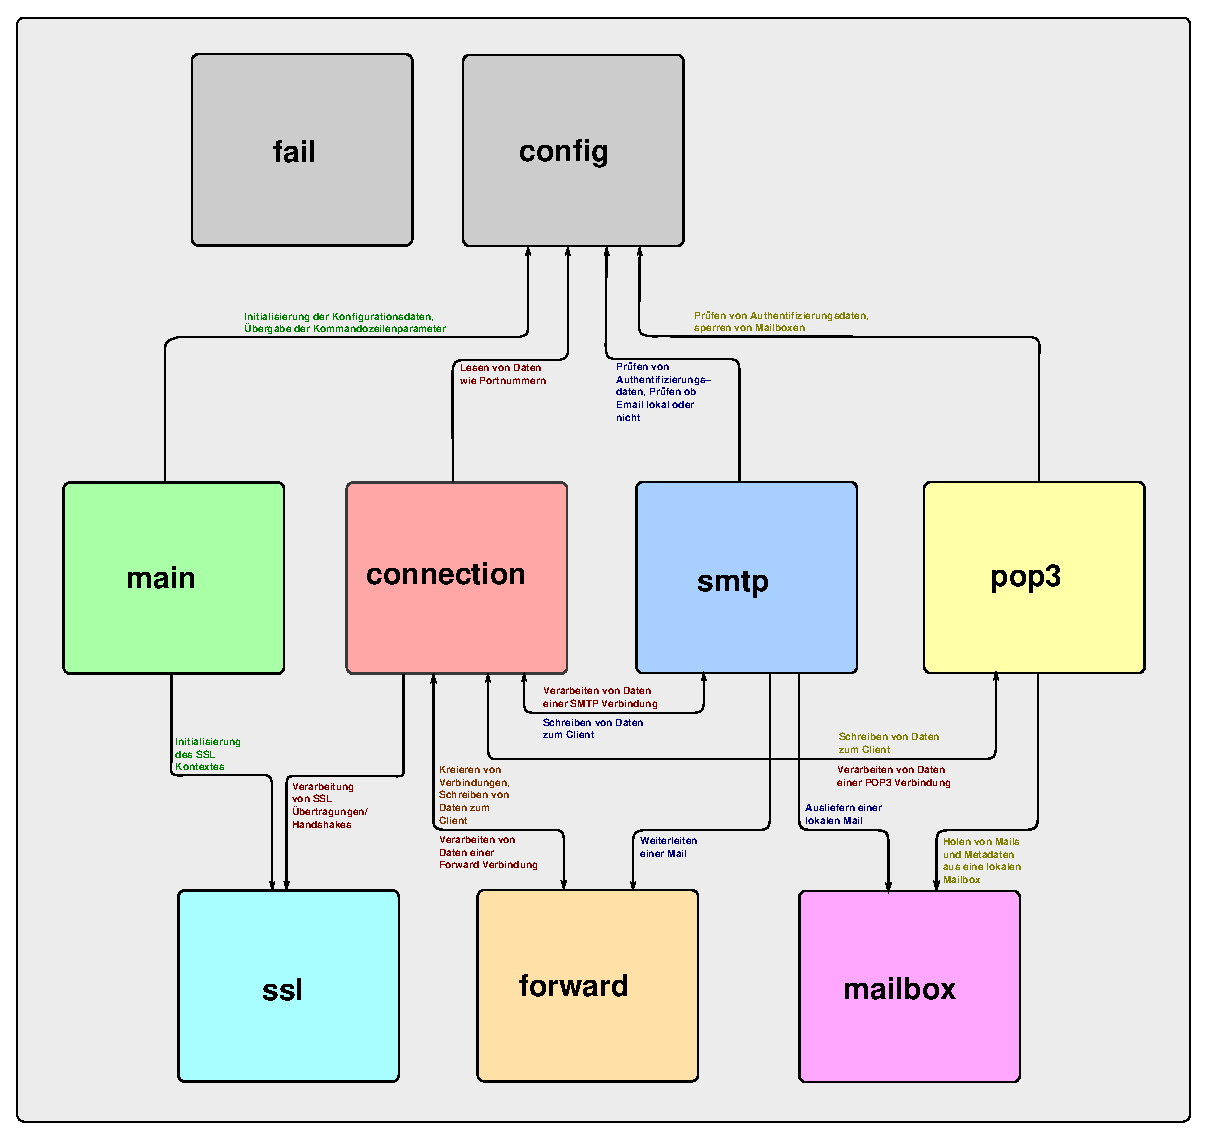
\includegraphics[width=\textwidth]{schema.eps}
    \caption{Modulschema}
    \label{fig:schema}
  \end{figure}
\end{appendix}
\end{document}
